\documentclass[a4paper,11pt,fleqn]{article}%fleqn pour aligner les equations à gauche
\usepackage{../../Styles/Exercice}


\newcommand{\chnum}{Chapitre 11}
\newcommand{\chtitle}{Décrire un mouvement}
\newcommand{\dtype}{Exercices}
  
\begin{document}
\maketitle

\begin{multicols}{2}
\section{La route du rhum}
L'orthodromie (route la plus courte formant un arc de cercle) reliant Saint-Malo à Pointe -à-Pitre est dessinée ci après. Elle est de \SI{3452}{M} (le symbole M signifiant mille marin). En 2018, Francis Joyon bat le record de la traversée en 7j 14h et 47s à la vitesse moyenne de \SI{23,95}{nd}, le symbole (nd) signifiant n\oe ud.
\begin{enumerate}
	\item Parcourue à vitesse constante, décrire cette trajectoire dans le référentiel géocentrique.
	\item Rechercher sur Internet la valeur d'un mile marin (M).
	\item Préciser si le trajet suivi par le skipper est orthodromique.
\end{enumerate}

\section{Conditions initiales d'un mouvement}
Les trois schémas ci-dessous représentent les conditions initiales de trois mouvements.\\
Déterminer les coordonnées des vecteurs vitesse initiales et accélération pour les trois situations représentées ci-dessous.

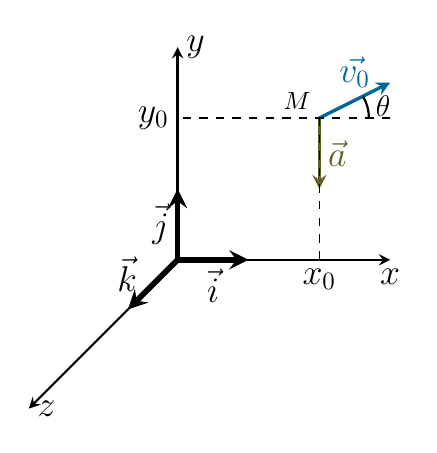
\begin{tikzpicture}[scale=.9, transform shape]
	\draw[thick, -stealth] (0,0) -- (0,3);
	\draw[thick, -stealth] (0,0) -- (3,0);
	\draw[thick, -stealth] (0,0) -- (-2.1,-2.1);
	
	\draw[line width = 2pt, -stealth] (0,0) to (1,0);
	\draw[line width = 2pt, -stealth] (0,0) to (0,1);
	\draw[line width = 2pt, -stealth] (0,0) to (-.7,-.7);
	
	\node[right] (y) at (0,3){\Large $y$};
	\node[below] (x) at (3,0){\Large $x$};
	\node[right] (z) at (-2.1,-2.1){\Large $z$};
	
	\node[left] (j) at (0,.5){\Large $\vec{j}$};
	\node[below] (i) at (.5,0){\Large $\vec{i}$};
	\node[left] (k) at (-.45,-.2){\Large $\vec{k}$};
	
	\node[above left] (M) at (2,2){$M$};
	\draw[line width = 1.2pt, olive!60!black,-stealth] (2,2) to (2,1);
	\draw[line width = 1.2pt, blue!60!green,-stealth] (2,2) to (3,2.5);
	\draw[dashed] (2,2) -- (2,0);
	\draw[dashed] (3,2) -- (0,2);
	
	\node[left] (y0) at (0,2){\Large $y_0$};
	\node[below] (x0) at (2,0){\Large $x_0$};
	
	\node[right,olive!60!black] (a) at (2,1.5){\Large $\vec{a}$};
	\node[above,blue!60!green] (v0) at (2.5,2.3){\Large $\vec{v_0}$};
	\node[above] (theta) at (2.9,1.9){\large $\theta$};
	
	\draw[thick] (2.7,2) arc (0:30:.6);
\end{tikzpicture}

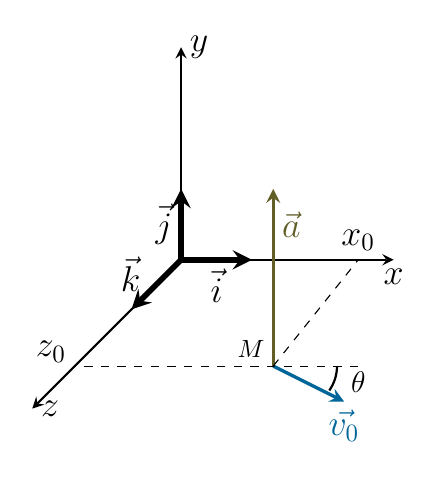
\begin{tikzpicture}[scale=.9, transform shape]
	\draw[thick, -stealth] (0,0) -- (0,3);
	\draw[thick, -stealth] (0,0) -- (3,0);
	\draw[thick, -stealth] (0,0) -- (-2.1,-2.1);
	
	\draw[line width = 2pt, -stealth] (0,0) to (1,0);
	\draw[line width = 2pt, -stealth] (0,0) to (0,1);
	\draw[line width = 2pt, -stealth] (0,0) to (-.7,-.7);
	
	\node[right] (y) at (0,3){\Large $y$};
	\node[below] (x) at (3,0){\Large $x$};
	\node[right] (z) at (-2.1,-2.1){\Large $z$};
	
	\node[left] (j) at (0,.5){\Large $\vec{j}$};
	\node[below] (i) at (.5,0){\Large $\vec{i}$};
	\node[left] (k) at (-.45,-.2){\Large $\vec{k}$};
	
	\node[above left] (M) at (1.3,-1.5){$M$};
	\draw[line width = 1.2pt, olive!60!black,-stealth] (1.3,-1.5) to (1.3,1);
	\draw[line width = 1.2pt, blue!60!green,-stealth] (1.3,-1.5) to (2.3,-2);
	\draw[dashed] (2.5,-1.5) -- (-1.5,-1.5);
	\draw[dashed] (1.3,-1.5) -- (2.5,0);
	
	\node[left] (z0) at (-1.5,-1.3){\Large $z_0$};
	\node[above] (x0) at (2.5,0){\Large $x_0$};
	
	\node[right,olive!60!black] (a) at (1.3,0.5){\Large $\vec{a}$};
	\node[below,blue!60!green] (v0) at (2.3,-2){\Large $\vec{v_0}$};
	\node[above] (theta) at (2.5,-2){\large $\theta$};
	
	\draw[thick] (2.2,-1.5) arc (0:-35:.6);
\end{tikzpicture}

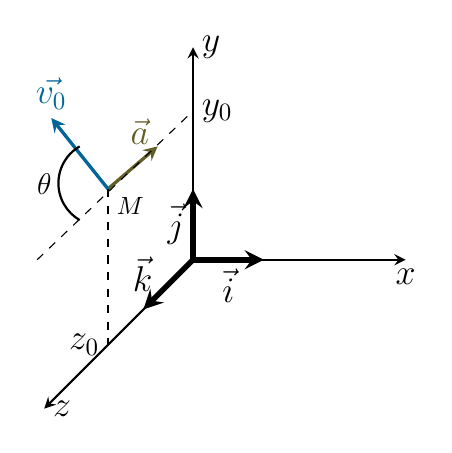
\begin{tikzpicture}[scale=.9, transform shape]
	\draw[thick, -stealth] (0,0) -- (0,3);
	\draw[thick, -stealth] (0,0) -- (3,0);
	\draw[thick, -stealth] (0,0) -- (-2.1,-2.1);
	
	\draw[line width = 2pt, -stealth] (0,0) to (1,0);
	\draw[line width = 2pt, -stealth] (0,0) to (0,1);
	\draw[line width = 2pt, -stealth] (0,0) to (-.7,-.7);
	
	\node[right] (y) at (0,3){\Large $y$};
	\node[below] (x) at (3,0){\Large $x$};
	\node[right] (z) at (-2.1,-2.1){\Large $z$};
	
	\node[left] (j) at (0,.5){\Large $\vec{j}$};
	\node[below] (i) at (.5,0){\Large $\vec{i}$};
	\node[left] (k) at (-.45,-.2){\Large $\vec{k}$};
	
	\node[below right] (M) at (-1.2,1){$M$};
	\draw[line width = 1.2pt, olive!60!black,-stealth] (-1.2,1) to (-.5,1.6);
	\draw[line width = 1.2pt, blue!60!green,-stealth] (-1.2,1) to (-2,2);
	\draw[dashed] (-2.2,0) -- (0,2.1);
	\draw[dashed] (-1.2,1) -- (-1.2,-1.2);
	
	\node[left] (z0) at (-1.2,-1.2){\Large $z_0$};
	\node[right] (y0) at (0,2.1){\Large $y_0$};
	
	\node[above,olive!60!black] (a) at (-.75,1.5){\Large $\vec{a}$};
	\node[above,blue!60!green] (v0) at (-2,2){\Large $\vec{v_0}$};
	\node[above] (theta) at (-2.1,.8){\large $\theta$};
	
	\draw[thick] (-1.6,1.6) arc (120:240:.6);
\end{tikzpicture}

\section{Aiguilles d'une horloge}
Une coccinelle se tient immobile sur l'aiguille des secondes d'une horloge. Cette aiguille mesure \SI{2,0}{cm}.
\begin{enumerate}
	\item Préciser le référentiel dans lequel la coccinelle est immobile.
	\item Donner la nature du mouvement de la coccinelle dans le référentiel des la pièce dans laquelle se trouve l'horloge.
	\item Préciser les caractéristiques des vecteurs vitesse et accélération de la coccinelle dans le référentiel de la pièce.
\end{enumerate}

\section{Chute de la tour Eiffel}
On étudie le mouvement d'un objet lâché depuis le troisième étage de la tour Eiffel, dont l'altitude au cours du temps est décrite par l'équation horaire suivante :
$$z(t) = -\dfrac{a}{2} \cdot t^2 + h_3$$
\begin{center}
	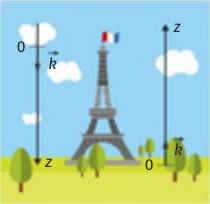
\includegraphics[scale=.6]{Ressources/TSPE_C4_Exercices_Fig1.png}
\end{center}
\begin{enumerate}
	\item Des deux repères représentés sur la photo, identifier celui choisi pour la modélisation de la coordonnée $z(t)$. Justifier.
	\item Déterminer la composante du vecteur vitesse $v_z(t)$.
	\item En déduire les normes des vitesses de l'objet au moment où il atteint la deuxième étage, puis le premier étage.
	\item Déterminer la durée de la chute jusqu'au sol.
\end{enumerate}
\noindent \colorbox{red!10}{
\begin{minipage}{.48\textwidth}
\textbf{Données :}\begin{itemize}
	\item \textbf{Hauteur du premier étage :} $h_1$ = \SI{58}{m}.
	\item \textbf{Hauteur du deuxième étage :} $h_2$ = \SI{116}{m}.
	\item \textbf{Hauteur du troisième étage :} $h_3$ = \SI{276}{m}.
	\item \textbf{Coefficient :} $a$ = \SI{9,8}{\meter\per\second\squared}
\end{itemize}
\end{minipage}}

\section{Mouvement rectiligne accéléré}
Un système, assimilé à un point $M$, se déplace le long d'un axe ($Ox$), en un mouvement rectiligne. On repère celui-ci par son abscisse $x(t)$ d'équation horaire : $$x(t) = -\dfrac{a}{2} \cdot t^2 + v_0 \cdot t + x_0$$
Ici, $a$ = \SI{8,0}{\meter\per\second\squared}, $v_0$ = \SI{16}{\meter\per\second} et $x_0$ = \SI{-5,0}{m}.
\begin{enumerate}
	\item Situer le système à l'instant initial $t_0$ = \SI{0}{s}.
	\item Exprimer le vecteur vitesse $\vec{v}(t)$ dans le repère ($O$, $\vec{i}$) et sa norme $v(t)$ en fonction du temps.
	\item Déterminer la date et la position d'arrêt du système.
	\item Calculer à quel instant le système passe par l'origine.
\end{enumerate}

\section{Mouvement rectiligne uniforme}
Un point mobile $M$ est suivi par enregistrement dans un repère ($O$, $\vec{i}$, $\vec{j}$). La modélisation de son mouvement fournit des équations horaires suivantes : $$x(t) = -v_0 \cdot t + x_0$$ $$y(t) = y_0$$ avec : $v_0$ = \SI{8}{\meter\per\second}, $x_0$ = \SI{4}{m} et $y_0$ = \SI{1}{m}.
\begin{enumerate}
	\item Exprimer les coordonnées du vecteur position initiale.
	\item Exprimer les coordonnées du vecteur vitesse et caractériser le mouvement.
	\item Calculer la vitesse du point $M$ en (-12m ; 1m).
\end{enumerate}

\section{Mouvement parabolique}
Un point $M$ adoptant une trajectoire parabolique admet comme équations horaires :
$$x(t)=v_{0x} \cdot t$$
$$y(t) = -\dfrac{a_y}{2} \cdot t^2 + v_{0y} \cdot t$$
avec : $v_{0x}$ = \SI{15,3}{\meter\per\second}, $a_y$ = \SI{9,81}{\meter\per\second\squared}, $v_{0y}$ = \SI{12,9}{\meter\per\second}.
\begin{enumerate}
	\item Exprimer les coordonnées du vecteur vitesse.
	\item Monter que la vitesse initiale du point $M$ vaut $v_0$ = \SI{20,0}{\meter\per\second}.
	\item En déduire l'angle $\alpha$ formé par le vecteur vitesse initiale $\vec{v_0}$ avec l'axe horizontal.
\end{enumerate}
\noindent \colorbox{red!10}{\begin{minipage}{.48\textwidth}
\textbf{Données : }\\
\textbf{Expression de la tangente de l'angle $\alpha$ :} $$\tan{(\alpha)} = \dfrac{v_{0y}}{v_{0x}}$$
\end{minipage}}

\begin{center}
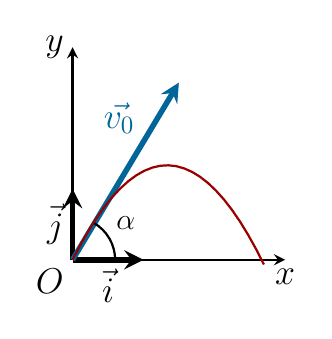
\begin{tikzpicture}[scale=.9, transform shape]
	\node[below left] (O) at (0,0){\Large $O$};
	\draw[thick, -stealth] (0,0) -- (0,3);
	\draw[thick, -stealth] (0,0) -- (3,0);
		
	\draw[line width = 2pt, -stealth] (0,0) to (1,0);
	\draw[line width = 2pt, -stealth] (0,0) to (0,1);
	
	\node[left] (y) at (0,3){\Large $y$};
	\node[below] (x) at (3,0){\Large $x$};
		
	\node[left] (j) at (0,.5){\Large $\vec{j}$};
	\node[below] (i) at (.5,0){\Large $\vec{i}$};
	
	%\draw[line width = 1.2pt, blue!60!green,-stealth] (-1.2,1) to (-2,2);
	
	\node[left,blue!60!green] (v0) at (1,2){\Large $\vec{v_0}$};
	\node[above] (alpha) at (.75,0.3){\large $\alpha$};
	
	\draw[line width = 2pt, -stealth, blue!60!green] (0,0) to (1.5,2.5);
	
	\draw[thick] (0.6,0) arc (0:60:.6);
	\draw [domain=0:2.7, thick, red!60!black] plot(\x,{-0.75*\x * \x  + 2*\x});
\end{tikzpicture}
\end{center}
\section{Mouvement circulaire}
Un point $M$ décrit une trajectoire dont les équations horaires de position sont : $$x(t) = R \cdot \cos{(\omega \cdot t)}$$
$$y(t) = R \cdot \sin{(\omega \cdot t)}$$
avec $R$ = \SI{2}{m}, $\omega$ = \SI{2}{\radian\per\second}.
\begin{enumerate}
	\item Montrer que la trajectoire est circulaire.
	\item Déterminer les caractéristiques du vecteur vitesse à $t_0$ = \SI{0}{s}.
\end{enumerate}
\noindent \colorbox{red!10}{\begin{minipage}{.48\textwidth}
\textbf{Données : }\\
\textbf{Équation d'un cercle de centre O (0m ; 0m) : } $$x^2 + y^2 = R^2$$
\textbf{Dérivées usuelles :} $$\cos{(u)}' = -u'\cdot \sin{(u)}$$
$$\sin{(v)'} = v' \cdot \cos{(v)}$$
\end{minipage}}

\section{Ballon-sonde}
\noindent \colorbox{orange!10}{\begin{minipage}{.48\textwidth}
\textbf{Définition}\\
Un ballon-sonde est un ballon à gaz utilisé dans les domaines de la météorologie et de l'astronautique. Il s'agit d'un ballon libre non habité, utilisé pour faire des mesures locales dans l'atmosphère grâce à un certain nombre d'instruments à bord, dans une nacelle appelée radiosonde. Le ballon-sonde a été inventé par Gustavo Hermite en 1892.\\
Son principal intérêt est de pouvoir atteindre des altitudes d'au moins \SI{35}{km}, le record étant à \SI{53}{km}, difficile à obtenir avec des moyens plus conventionnels tels que les avions, et à un coût bien inférieur à une fusée-sonde ou un satellite.
\end{minipage}}

Lors d'un lâcher, un ballon -sonde a une vitesse verticale constante $v_0$ tout au long de son ascension. Le vent emporte le ballon-sonde à la vitesse horizontale $v_x(t) = k \cdot z(t)$, proportionnelle à l'altitude du ballon.\\
L'étude du mouvement du centre du ballon-sonde s'effectue dans le repère galiléen ($O$, $\vec{i}$, $\vec{k}$).
\begin{enumerate}
	\item Déterminer l'équation horaire $z(t)$.
	\item À l'aide de $v_x(t)$, déterminer $x(t)$.
	\item Déterminer les composantes du vecteur accélération.
\end{enumerate}

\section{Lancer de poids}
Lors des Championnats du monde d'athlétisme qui ont eu lieu à Paris en août 2003, le vainqueur de l'épreuve du lancer du poids, Andrei Mikhnevich, a réussi un jet à une distance $d$ = \SI{21,69}{m}.\\
L'entraîneur de l'un de ses concurrents souhaite étudier ce lancer. Pour cela, il dispose pour le centre d'inertie du boulet, en plus de la valeur \SI{21,69}{m} du recors, de la vitesse initiale $v_0$ mesurée à l'aide d'un cinémomètre et de l'altitude $h$.\\
L'entraîneur a étudié le mouvement du boulet et a obtenu trois graphiques :
\begin{itemize}
	\item Le graphique de la trajectoire $y=f(x)$ du boulet
	\item les graphes de $v_x(t)$ et de $v_y(t)$ en fonction du temps $t$ où $v_x(t)$ et $v_y(t)$ sont les coordonnées horizontales et verticales du vecteur vitesse $\vec{v}(t)$.
\end{itemize}

\noindent \colorbox{red!10}{\begin{minipage}{.48\textwidth}
\textbf{Données : }
\begin{itemize}
	\item \textbf{Vitesse initiale du boulet : } $v_0$ = \SI{13,8}{\meter\per\second}
	\item \textbf{Hauteur initiale du lancer :} $h$ = \SI{2,62}{m}
	\item \textbf{Intensité de pesanteur :} $g$ = \SI{9,81}{\newton\per\kilo\gram}
\end{itemize}
\end{minipage}}

\begin{center}
	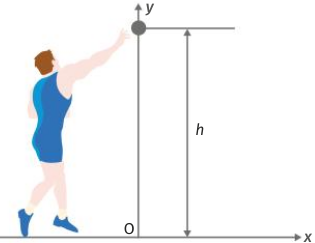
\includegraphics[scale=.7]{Ressources/TSPE_C4_Exercices_Fig2.png}
	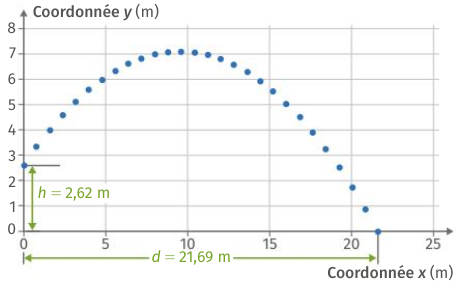
\includegraphics[scale=.75]{Ressources/TSPE_C4_Exercices_Fig3.png}
\end{center}

\end{multicols}
\end{document}